\section{Corpus Construction}

\subsection{Extraction}
\begin{frame}
    \frametitle{Extraction}

    \begin{itemize}
        \item Humorous: we looked in Twitter for the keyword \emph{chistes} and choose accounts, reaching 16,488 tweets.
        \item Non humorous: news, philosophical phrases and curiosities facts accounts, summing 22,875 tweets.
    \end{itemize}
\end{frame}

\subsection{Annotation}
\begin{frame}
    \frametitle{Annotation}

    \begin{itemize}
        \item Naturally we should tag the tweets according to the type of account, but there are lots of inconsistencies.

        \begin{itemize}
            \item Example: \emph{RT @MichelPesquera: El significado de ``Nada'' http://t.co/L1e2uHOhM4}

            \item They have to be cured by hand.
        \end{itemize}

        \item But it's an excesive amount of tweets to classify.

        \begin{itemize}
            \item So we created an app to allow anyone to anotate.
        \end{itemize}
    \end{itemize}

    \vspace{1cm}

    \begin{center}
        \bf
        Humor is crowd-defined.
    \end{center}
\end{frame}

\begin{frame}
\frametitle{Annotation}
\framesubtitle{Classes to consider}
        \begin{center}
        \begin{columns}[c]
            \begin{column}[c]{0.50\textwidth}
                \centering
                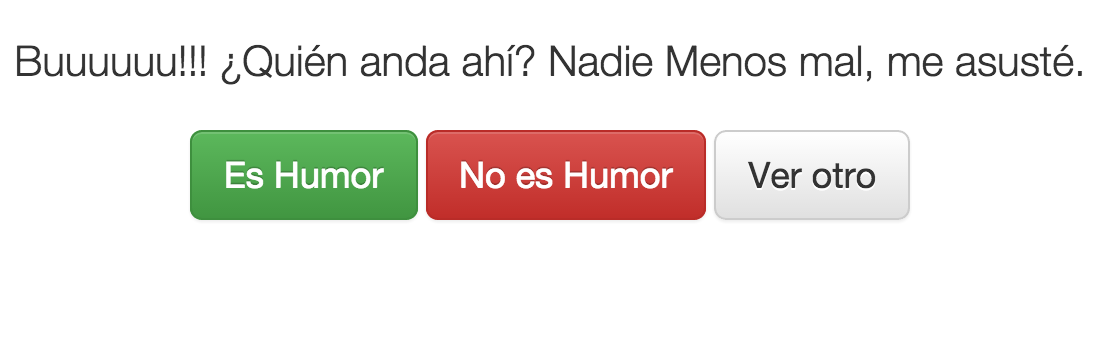
\includegraphics[frame, height=1.8cm, width=5.5cm]{pagina-dos-opciones.png}
            \end{column}

            \begin{column}[c]{0.50\textwidth}
                \centering
                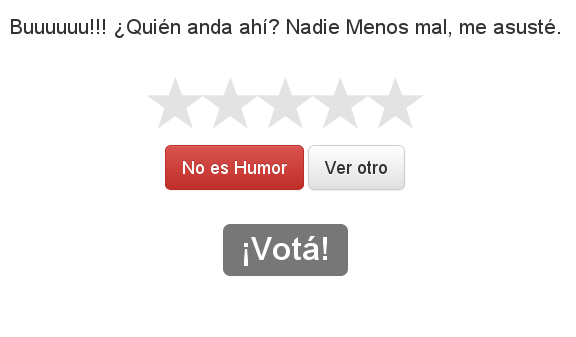
\includegraphics[frame, height=3.5cm, width=5.5cm]{pagina.png}
            \end{column}
        \end{columns}
    \end{center}
\end{frame}
\begin{frame}
    \frametitle{Annotation}
    \framesubtitle{Other considerations}

    \begin{itemize}
        \item Explicit content

        \begin{itemize}
            \item We are looking for the largest number of annotators.
            \item So explicit content is removed.
        \end{itemize}

        \item Performance

        \begin{itemize}
            \item Low-latency
            \item Time between tweets
        \end{itemize}

        \item Selection algorithm

        \begin{itemize}
            \item Random
            \item Without repetition
        \end{itemize}
    \end{itemize}
\end{frame}
\begin{frame}
\frametitle{Annotation}
\framesubtitle{Final app}
    \begin{center}
        \begin{columns}[c]
            \begin{column}[c]{0.45\textwidth}
                \centering
                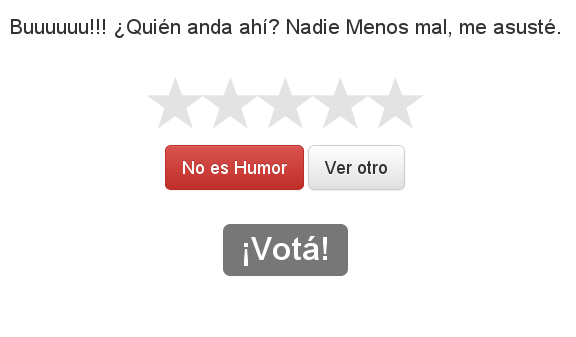
\includegraphics[frame, height=3.5cm]{pagina.png}
            \end{column}

            \begin{column}[c]{0.45\textwidth}
                \centering
                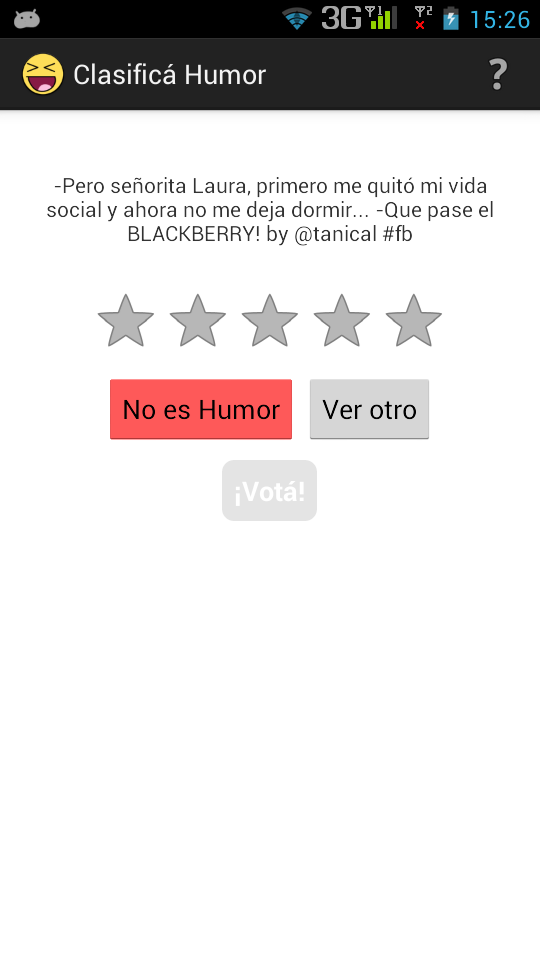
\includegraphics[frame, height=7cm]{app.png}
            \end{column}
        \end{columns}
    \end{center}
\end{frame}

\subsubsection{Annotation results}
\begin{frame}[allowframebreaks]
    \frametitle{Annotation results}

    \begin{itemize}
        \item[+] 60k votes
        \item[--] 20k removed votes
        \item[--] 6,5k ``skip'' votes
        \item[=] 33,5k considered votes
    \end{itemize}

    \framebreak{}

    \begin{center}
        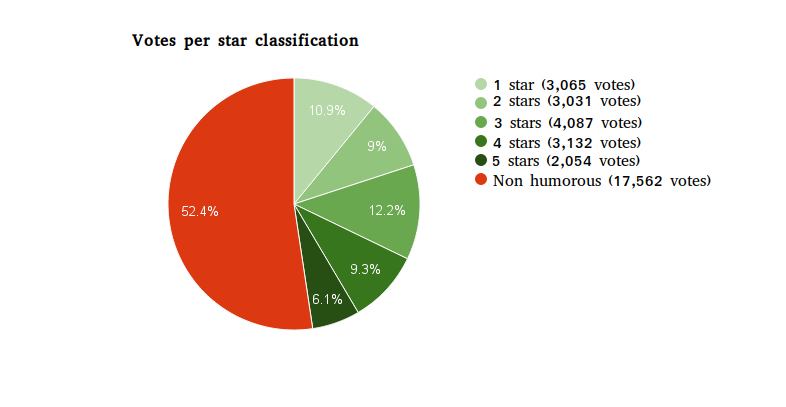
\includegraphics{votos_por_calificacion_torta.png}

        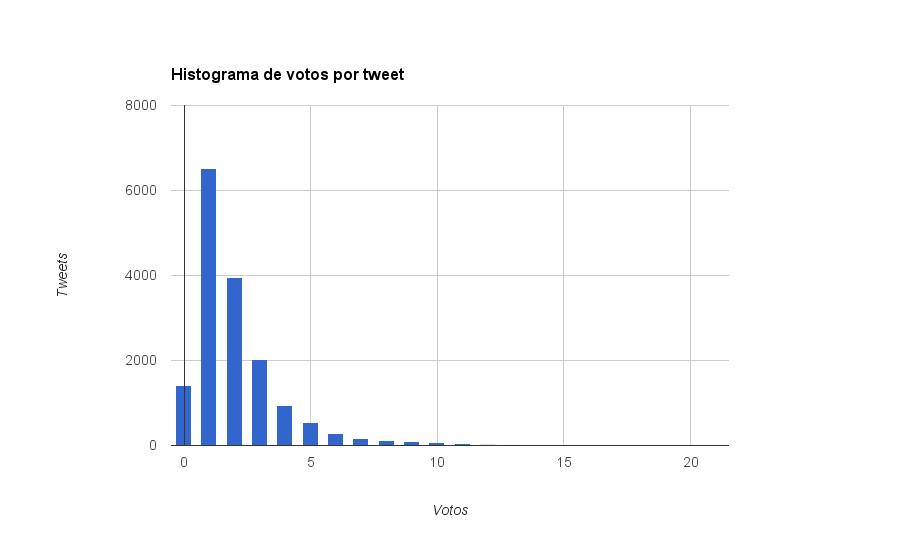
\includegraphics{histograma.png}
    \end{center}
\end{frame}

\subsubsection{Humor among voters}

\begin{frame}[allowframebreaks]
    \frametitle{Humor among voters}

    Rate of positive votes: $\frac{\#\{positive\ votes\}}{\#\{total\}}$ % chktex 21

    \begin{center}
        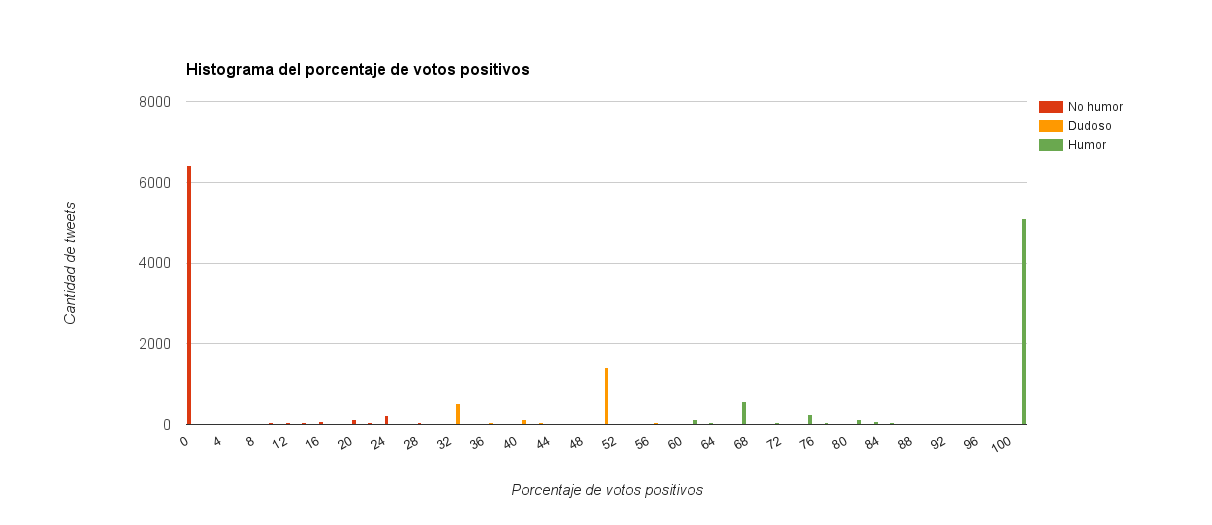
\includegraphics[height=3.75cm]{histograma_porcentaje_humor.png}
    \end{center}

    \begin{itemize}
        \item $[60\%, 100\%] \Rightarrow$ \textbf{Humor}
        \item $(30\%, 60\%) \Rightarrow$ \textbf{Doubtful}
        \item $[0\%, 30\%] \Rightarrow$ \textbf{Non humorous}
    \end{itemize}

    \framebreak{}

    \begin{center}
        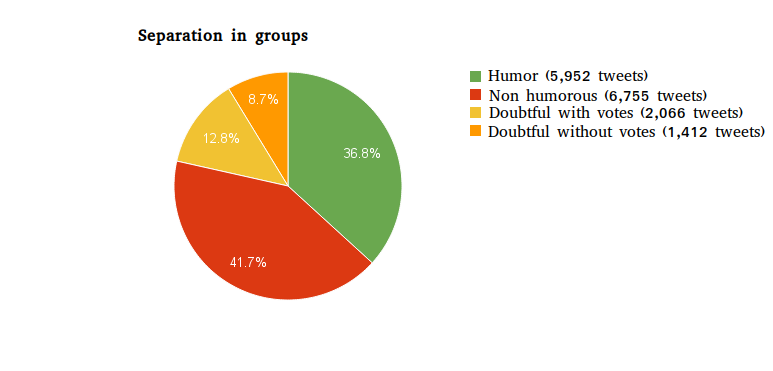
\includegraphics[height=6cm]{grupos.png}
    \end{center}
\end{frame}

\subsubsection{Agreement between annotators}

\begin{frame}[allowframebreaks]
    \frametitle{Agreement between annotators}

    \begin{itemize}
        \item We wanted to know what was the agreement between people.
        \item Fleiss' kappa was used.
        \item It measures the votes against a random one, being 1 the best possible and 0 being equal to random.
    \end{itemize}

    \note{Interesa saber cuál fue la concordancia entre los anotadores, es decir, qué tan de acuerdo estuvo la gente a la hora de anotar como humor (1, 2, 3, 4 o 5 estrellas) o como humorístico a los tweets. Se propone utilizar la medida kappa. Esta medida se fija la cantidad de pares de anotadores que están de acuerdo en cada categoría para cada tweet. El resultado es un número, en donde 0 significa una anotación hecha al azar y 1 es el mejor acuerdo posible.}

    \framebreak{}

    \begin{itemize}
        \item 0.416 for tweets with 2 votes, that are 4,011.

        \item 0.325 for tweets with 6 votes, that are 278.

        \item Mid level agreement.

        \begin{itemize}
            \item There's clearly no unanimity.
        \end{itemize}
    \end{itemize}
\end{frame}
